\documentclass[aspectratio=169,10pt]{beamer}

% ============================================================
%  Curso de Maestría — Métodos de Optimización
%  Clase 2: Métodos de búsqueda determinísticos y básicos
%           (bisección, áurea, grid search, random walk, Nelder-Mead)
% ============================================================

\usepackage[utf8]{inputenc}
\usepackage[T1]{fontenc}
\usepackage{lmodern}
\usepackage[spanish]{babel}
\usepackage{amsmath,amssymb,amsthm}
\usepackage{graphicx}
\usepackage{booktabs}
\usepackage{xcolor}
\usepackage{listings}
\usepackage{tikz}

\graphicspath{{figs/}}

\usetheme{metropolis}
\metroset{block=fill, progressbar=frametitle, sectionpage=progressbar, numbering=fraction}

\definecolor{pygreen}{RGB}{0,128,0}
\definecolor{pyblue}{RGB}{0,0,180}
\definecolor{pygray}{RGB}{110,110,110}
\definecolor{codebg}{RGB}{245,245,245}

\lstdefinestyle{pythonstyle}{
  language=Python,
  backgroundcolor=\color{codebg},
  basicstyle=\ttfamily\scriptsize,
  keywordstyle=\color{pyblue}\bfseries,
  commentstyle=\color{pygreen}\itshape,
  stringstyle=\color{pygray},
  numbers=none,
  breaklines=true,
  showstringspaces=false,
  frame=single,
  rulecolor=\color{gray!40},
  xleftmargin=4pt,
  xrightmargin=4pt,
  aboveskip=6pt,
  belowskip=2pt,
}
\lstset{style=pythonstyle}

% --- notación abreviada ---
\newcommand{\R}{\mathbb{R}}
\newcommand{\grad}{\nabla}
\newcommand{\x}{\mathbf{x}}

\title{Métodos de Optimización}
\subtitle{Clase 2: Métodos de búsqueda determinísticos y básicos}
\author{[Nombre del profesor]}
\institute{Programa de Maestría, [Nombre de la universidad / programa]}
\date{Septiembre de 2026}

\begin{document}

% ---------------------------------------------------------------
\begin{frame}[plain]
  \maketitle
\end{frame}

\begin{frame}{Contenido}
  \footnotesize
  \begin{columns}[T]
    \column{0.5\textwidth}
    \begin{enumerate}
      \setcounter{enumi}{0}
      \item Motivación: ¿por qué buscar si ya vimos condiciones analíticas?
      \item Bisección en 1D
      \item Búsqueda áurea en 1D
      \item Bisección vs.\ áurea
      \item Búsqueda exhaustiva (grid search) en 1, 2 y 3 variables
    \end{enumerate}
    \column{0.5\textwidth}
    \begin{enumerate}
      \setcounter{enumi}{5}
      \item Random walk en 2D
      \item Nelder--Mead (amoeba) en 2D
      \item Síntesis y tabla comparativa
      \item Vista previa: Clase 3
      \item Ejercicios y referencias
    \end{enumerate}
  \end{columns}
\end{frame}

% ==================================================================
\section{Motivación}
% ==================================================================

\begin{frame}{¿Por qué necesitamos métodos de búsqueda?}
  En la Clase 1 vimos condiciones \textbf{analíticas}: resolver
  $\grad f(\x)=\mathbf 0$, clasificar con la Hessiana, usar Lagrange/KKT.
  Todo eso requiere que $f$ sea \textbf{diferenciable} y que podamos
  \textbf{resolver el sistema de ecuaciones} resultante.
  \begin{alertblock}{¿Qué pasa si...?}
    \begin{itemize}
      \item no conocemos una fórmula cerrada para $f$ (es una simulación,
        un experimento, una caja negra)?
      \item $f$ no es diferenciable, o su derivada es muy costosa/imposible
        de calcular?
      \item $\grad f(\x)=\mathbf 0$ no se puede resolver algebraicamente?
      \item $f$ tiene muchísimos mínimos locales y no confiamos en que el
        descenso de gradiente encuentre el bueno?
    \end{itemize}
  \end{alertblock}
  Hoy: métodos que solo necesitan \textbf{evaluar} $f$ (a veces $f'$), sin
  resolver ecuaciones. Empezamos por los más simples y deterministas.
\end{frame}

\begin{frame}{El menú de hoy}
  \begin{columns}
    \column{0.5\textwidth}
    \textbf{1 variable}
    \begin{itemize}
      \item Bisección (usa $f'$)
      \item Búsqueda áurea (no usa $f'$)
    \end{itemize}
    \vspace{0.3cm}
    \textbf{Cualquier número de variables}
    \begin{itemize}
      \item Búsqueda exhaustiva (grid search)
    \end{itemize}
    \column{0.5\textwidth}
    \textbf{2 (o más) variables, sin derivadas}
    \begin{itemize}
      \item Random walk
      \item Nelder--Mead (amoeba)
    \end{itemize}
  \end{columns}
  \vspace{0.4cm}
  \begin{block}{}
    Todos son \textbf{deterministas} o casi (random walk tiene una parte
    aleatoria, pero es el más simple posible). En la \textbf{Clase 3}
    veremos metaheurísticas más sofisticadas que combinan aleatoriedad
    con reoptimización: basin hopping, simulated annealing, algoritmos
    genéticos y particle swarm.
  \end{block}
  \small Cada método se muestra con \textbf{código manual} (para entender
  el mecanismo) y su \textbf{equivalente en scipy} (para comparar contra
  una implementación profesional).
\end{frame}

% ==================================================================
\section{Bisección en 1D}
% ==================================================================

\begin{frame}{Bisección para minimizar: la idea}
  \begin{block}{Idea}
    Un mínimo de $f$ diferenciable es una \textbf{raíz de $f'$}. Si
    tenemos $[a,b]$ con $f'(a)$ y $f'(b)$ de signos opuestos (uno negativo,
    uno positivo), sabemos que hay un mínimo adentro — y podemos usar
    \textbf{bisección clásica sobre $f'$} para encontrarlo.
  \end{block}
  \begin{block}{Algoritmo}
    \begin{enumerate}
      \item $c = (a+b)/2$; evaluar $f'(c)$.
      \item Si $f'(c)$ tiene el mismo signo que $f'(a)$: $a\leftarrow c$.
        Si no: $b\leftarrow c$.
      \item Repetir hasta que $b-a$ sea suficientemente chico.
    \end{enumerate}
  \end{block}
  \begin{alertblock}{Convergencia}
    \textbf{Lineal}: el intervalo se reduce a la \textbf{mitad} en cada
    iteración, garantizado, sin importar qué tan fea sea $f$ (mientras
    cumpla la condición de signos). Necesita poder evaluar $f'$.
  \end{alertblock}
\end{frame}

\begin{frame}[fragile]{Bisección: ejemplo paso a paso}
  $f(x)=x^2-2x+3$, $f'(x)=2x-2$ (la misma función de la Clase 1, mínimo
  exacto en $x^*=1$). Intervalo inicial $[-2,5]$: $f'(-2)=-6<0$,
  $f'(5)=8>0$. Primeras iteraciones reales:
  \tiny
\begin{lstlisting}
it= 1  a=-2.000000  b= 5.000000  c= 1.500000  f'(c)= 1.000000  ancho=7.000000
it= 2  a=-2.000000  b= 1.500000  c=-0.250000  f'(c)=-2.500000  ancho=3.500000
it= 3  a=-0.250000  b= 1.500000  c= 0.625000  f'(c)=-0.750000  ancho=1.750000
it= 4  a= 0.625000  b= 1.500000  c= 1.062500  f'(c)= 0.125000  ancho=0.875000
it= 5  a= 0.625000  b= 1.062500  c= 0.843750  f'(c)=-0.312500  ancho=0.437500
      ...
it=22  ancho=0.0000033  ->  x* = 1.000000   f(x*) = 2.000000
\end{lstlisting}
  \normalsize
  22 iteraciones para reducir el intervalo a $3.3\times10^{-6}$ — cada
  iteración exactamente a la mitad de la anterior: $7\times0.5^{22}\approx
  1.7\times10^{-6}$, consistente con lo observado.
\end{frame}

\begin{frame}[fragile]{Bisección: código}
  \begin{columns}
    \column{0.52\textwidth}
    \textbf{Manual:}
\begin{lstlisting}
def biseccion_min(fprime, a, b, tol=1e-6):
    while True:
        c = 0.5*(a + b)
        fc = fprime(c)
        if abs(fc) < tol or (b-a) < tol:
            return c
        if np.sign(fc) == np.sign(fprime(a)):
            a = c
        else:
            b = c
\end{lstlisting}
    \column{0.48\textwidth}
    \textbf{Con scipy:}
\begin{lstlisting}
from scipy.optimize import brentq

x_star = brentq(fprime, a, b, xtol=1e-6)
\end{lstlisting}
    \small \texttt{brentq} resuelve el mismo problema
    (raíz de $f'$) pero combina secante e
    interpolación cuadrática inversa con
    bisección — converge \textbf{mucho} más
    rápido que bisección pura, garantizando
    robustez.
  \end{columns}
  \vspace{0.3cm}
  Ambos dan $x^*=1.000000$, $f(x^*)=2.000000$. Script completo:
  \texttt{scripts/01\_biseccion\_1d.py}
\end{frame}

% ==================================================================
\section{Búsqueda áurea en 1D}
% ==================================================================

\begin{frame}{Búsqueda áurea: la idea}
  \begin{block}{Idea}
    A diferencia de bisección, \textbf{no usa $f'$} — solo evalúa $f$.
    Sirve para cualquier función \textbf{unimodal} (un solo mínimo) en
    $[a,b]$, incluso si no es diferenciable.
  \end{block}
  \begin{block}{Algoritmo}
    Mantiene $[a,b]$ con dos puntos interiores $x_1<x_2$ colocados con la
    razón áurea $\varphi=\frac{\sqrt5-1}{2}\approx0.618$:
    \begin{itemize}
      \item Si $f(x_1)<f(x_2)$: el mínimo está en $[a,x_2]$ — descartamos
        la derecha.
      \item Si $f(x_1)>f(x_2)$: el mínimo está en $[x_1,b]$ — descartamos
        la izquierda.
    \end{itemize}
  \end{block}
  \begin{alertblock}{La razón áurea no es casualidad}
    Con esa proporción, uno de los dos puntos interiores \textbf{se
    reutiliza} de la iteración anterior — cada paso necesita solo
    \textbf{una} evaluación nueva de $f$, no dos.
  \end{alertblock}
\end{frame}

\begin{frame}[fragile]{Búsqueda áurea: ejemplo paso a paso}
  Mismo problema: $f(x)=x^2-2x+3$ en $[-2,5]$.
  \tiny
\begin{lstlisting}
it= 1  a=-2.00  b= 5.00  x1= 0.674 x2= 2.326  f(x1)=2.106  f(x2)=3.759  ancho=7.000
it= 2  a=-2.00  b= 2.33  x1=-0.348 x2= 0.674  f(x1)=3.816  f(x2)=2.106  ancho=4.326
it= 3  a=-0.35  b= 2.33  x1= 0.674 x2= 1.305  f(x1)=2.106  f(x2)=2.093  ancho=2.674
it= 4  a= 0.67  b= 2.33  x1= 1.305 x2= 1.695  f(x1)=2.093  f(x2)=2.483  ancho=1.652
      ...
it=34  ancho=0.00000089  ->  x* = 1.000000   f(x*) = 2.000000
\end{lstlisting}
  \normalsize
  \textbf{34 iteraciones} (vs.\ 22 de bisección) para la misma tolerancia:
  áurea reduce el intervalo por un factor $\varphi\approx0.618$ por
  iteración (más lento que el $0.5$ de bisección), pero a cambio
  \textbf{no necesita derivada}.
\end{frame}

\begin{frame}[fragile]{Búsqueda áurea: código}
  \begin{columns}
    \column{0.55\textwidth}
    \textbf{Manual (núcleo del bucle):}
\begin{lstlisting}
PHI = (5**0.5 - 1) / 2   # ~0.618
x1 = b - PHI*(b-a); x2 = a + PHI*(b-a)
f1, f2 = f(x1), f(x2)
while (b - a) > tol:
    if f1 < f2:
        b = x2; x2, f2 = x1, f1
        x1 = b - PHI*(b-a); f1 = f(x1)
    else:
        a = x1; x1, f1 = x2, f2
        x2 = a + PHI*(b-a); f2 = f(x2)
\end{lstlisting}
    \column{0.45\textwidth}
    \textbf{Con scipy:}
\begin{lstlisting}
from scipy.optimize import minimize_scalar

res = minimize_scalar(
    f, bracket=(a, (a+b)/2, b),
    method="golden")
\end{lstlisting}
    \small \texttt{scipy} implementa exactamente
    este algoritmo con ese nombre.
  \end{columns}
  \vspace{0.3cm}
  Script completo: \texttt{scripts/02\_busqueda\_aurea\_1d.py}
\end{frame}

% ==================================================================
\section{Bisección vs. áurea}
% ==================================================================

\begin{frame}{Bisección vs.\ búsqueda áurea}
  \begin{center}
    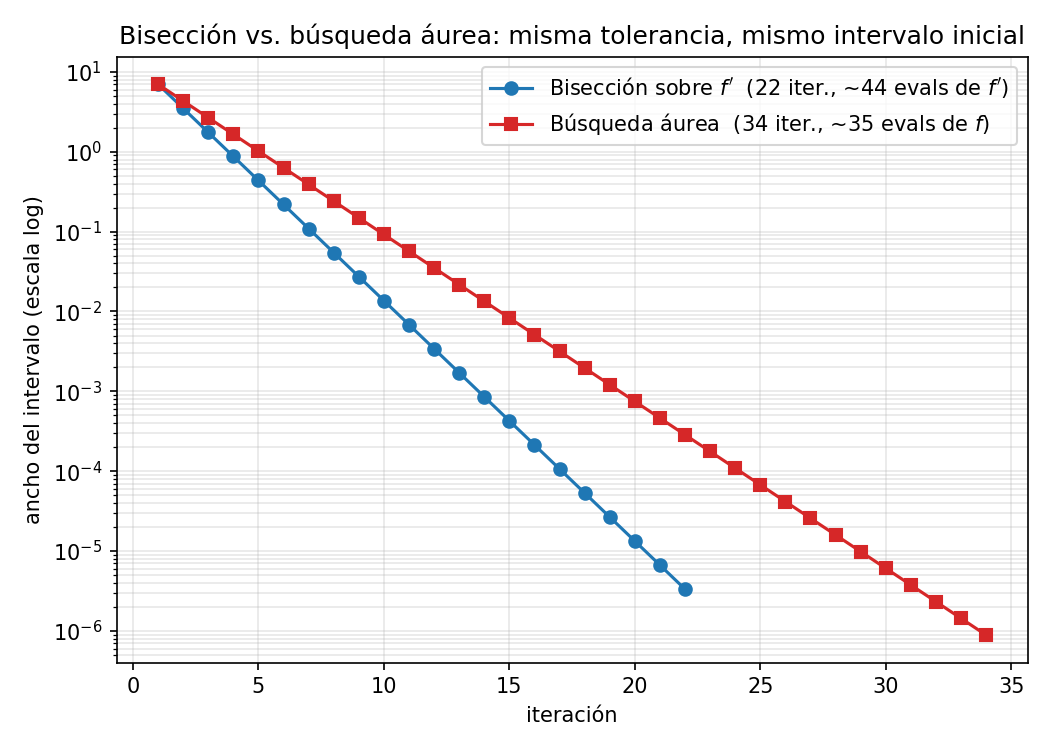
\includegraphics[height=6.2cm,keepaspectratio]{fig03_comparacion_biseccion_aurea.png}
  \end{center}
\end{frame}

\begin{frame}{¿Cuál usar?}
  \begin{block}{}
    \begin{itemize}
      \item Si $f'$ está disponible y es barata de evaluar:
        \textbf{bisección} (o mejor, un método tipo Brent que combina
        varias ideas) converge con menos iteraciones.
      \item Si $f$ no es diferenciable, o $f'$ es costosa/no disponible:
        \textbf{búsqueda áurea} es la opción segura — solo necesita
        evaluar $f$.
      \item Ambos requieren un intervalo inicial $[a,b]$ donde se sepa
        que hay un único mínimo (unimodalidad). Sin esa garantía, ninguno
        de los dos promete encontrar el mínimo \textbf{global}.
    \end{itemize}
  \end{block}
  \begin{alertblock}{Conexión con la Clase 1}
    Ambos son primos de los métodos de la Clase 1: bisección usa
    información de primer orden (el signo de $f'$, como la condición
    $\grad f=\mathbf 0$); áurea es puramente "evaluar y comparar", la
    filosofía que vamos a extender hoy a varias variables.
  \end{alertblock}
\end{frame}

% ==================================================================
\section{Búsqueda exhaustiva (grid search)}
% ==================================================================

\begin{frame}{Grid search: la idea}
  \begin{block}{Idea}
    Evaluar $f$ en \textbf{todos los puntos de una malla regular} y
    quedarse con el mejor. No requiere derivadas, no requiere que $f$ sea
    continua, \textbf{no le importa cuántos mínimos locales tenga} $f$ —
    siempre encuentra el mínimo \emph{de la malla}, que se acerca al
    mínimo real si la malla es suficientemente fina.
  \end{block}
  \begin{alertblock}{El precio: la maldición de la dimensionalidad}
    Con $N$ puntos por eje y $d$ variables, el costo es
    $N^d$ evaluaciones. Con $N=50$:
    \[
      d{=}1\to 50 \qquad d{=}2\to 2{,}500 \qquad d{=}3\to 125{,}000
      \qquad d{=}4\to 6{,}250{,}000 \ \dots
    \]
  \end{alertblock}
  Por eso grid search es práctico en 1--3 variables, y rápidamente
  inviable más allá.
\end{frame}

\begin{frame}[fragile]{Grid search en 1, 2 y 3 variables: código}
\begin{lstlisting}
# 1D: N evaluaciones
xs = np.linspace(-2, 5, N);  i = np.argmin(f1d(xs))

# 2D: N^2 evaluaciones
X, Y = np.meshgrid(np.linspace(-10,10,N), np.linspace(-10,10,N))
Z = f2d(X, Y);  idx = np.unravel_index(np.argmin(Z), Z.shape)

# 3D (o dD en general): N^d evaluaciones, con itertools.product
import itertools
mejor = min(itertools.product(xs3, ys3, zs3), key=lambda p: f3d(*p))
\end{lstlisting}
  \textbf{Con scipy:}
\begin{lstlisting}
from scipy.optimize import brute
res = brute(f2d, ranges, finish=None)        # grid puro
res = brute(f2d, ranges)                     # + pule con Nelder-Mead (default)
\end{lstlisting}
  Script completo: \texttt{scripts/04\_grid\_search\_1\_2\_3d.py}
\end{frame}

\begin{frame}{Grid search: resultado y costo}
  \begin{center}
    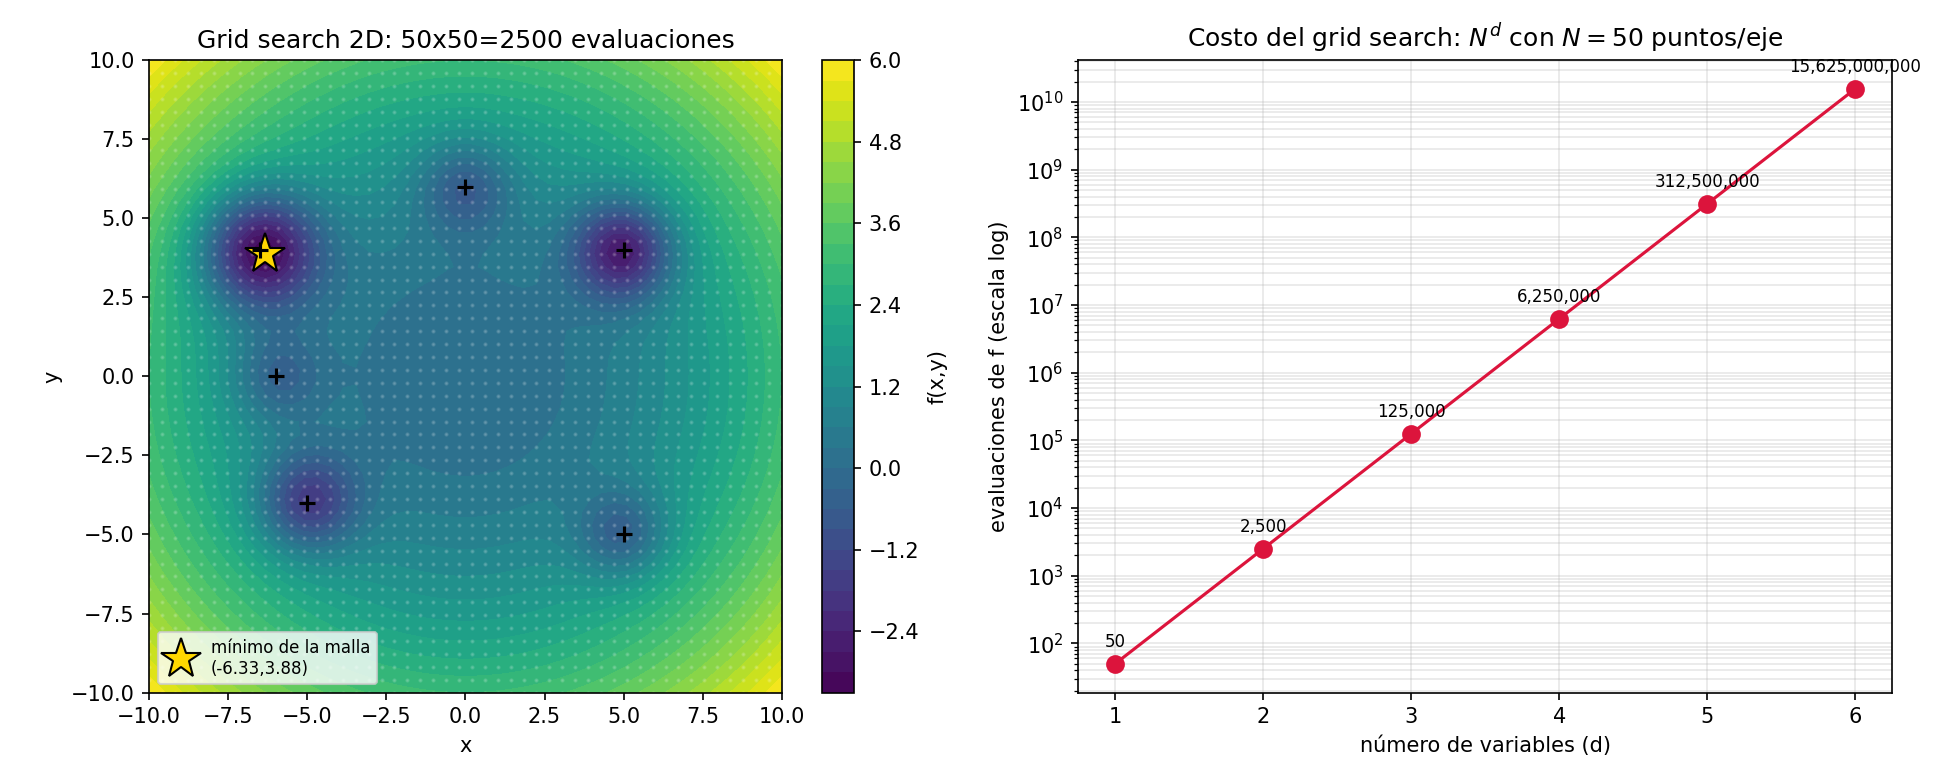
\includegraphics[width=0.92\textwidth,height=5.3cm,keepaspectratio]{fig04_grid_search.png}
  \end{center}
  \footnotesize Izquierda: malla $50\times50$ sobre un paisaje con 6
  mínimos locales — grid search encuentra el global sin ningún truco.
  Derecha: el costo $N^d$ crece brutalmente con la dimensión.
\end{frame}

\begin{frame}{Grid search: ventajas y límites}
  \begin{columns}
    \column{0.5\textwidth}
    \textbf{A favor}
    \begin{itemize}
      \item Encuentra el mínimo \textbf{global} de la malla, garantizado.
      \item No necesita nada sobre $f$: ni continuidad, ni convexidad,
        ni derivadas.
      \item Trivialmente paralelizable (cada evaluación es independiente).
    \end{itemize}
    \column{0.5\textwidth}
    \textbf{En contra}
    \begin{itemize}
      \item Costo $N^d$: inviable en más de 3--4 variables.
      \item La precisión está limitada por qué tan fina sea la malla.
      \item Desperdicia evaluaciones en zonas obviamente malas.
    \end{itemize}
  \end{columns}
  \vspace{0.3cm}
  \begin{alertblock}{Idea que retomaremos}
    Los métodos que siguen (random walk hoy; basin hopping, simulated
    annealing, GA, PSO en la Clase 3) tratan de \textbf{gastar las
    evaluaciones de forma más inteligente} que una malla uniforme.
  \end{alertblock}
\end{frame}

% ==================================================================
\section{Random walk en 2D}
% ==================================================================

\begin{frame}{Random walk: la idea}
  \begin{block}{Distinto de grid search y de Monte Carlo puro}
    Un \textbf{random walk} da un paso aleatorio \textbf{a partir del
    punto actual} — el recorrido es una cadena donde cada punto depende
    del anterior (a diferencia de grid search, que es una malla fija, y
    de random search/Monte Carlo, que muestrea puntos independientes en
    todo el dominio).
  \end{block}
  Dos variantes:
  \begin{itemize}
    \item \textbf{Greedy}: el paso solo se acepta si mejora $f$; si no,
      se descarta y se prueba otro paso aleatorio desde el mismo punto.
    \item \textbf{Puro}: el paso \textbf{siempre} se acepta, mejore o no
      — pura difusión, no converge a nada, solo explora.
  \end{itemize}
  \small Sin quererlo, ya estamos a un paso de simulated annealing
  (Clase 3): si en vez de "siempre" o "solo si mejora" usamos una
  probabilidad tipo Metrópolis, ahí aparece.
\end{frame}

\begin{frame}[fragile]{Random walk: código}
\begin{lstlisting}
def random_walk_greedy(f, x0, step=1.5, n_iter=500):
    x = np.array(x0, float);  fx = f(*x)
    for _ in range(n_iter):
        x_new = x + rng.uniform(-step, step, size=2)
        f_new = f(*x_new)
        if f_new < fx:                 # solo se mueve si MEJORA
            x, fx = x_new, f_new
    return x, fx

def random_walk_puro(f, x0, step=1.5, n_iter=500):
    x = np.array(x0, float);  x_best, f_best = x.copy(), f(*x)
    for _ in range(n_iter):
        x = x + rng.uniform(-step, step, size=2)   # SIEMPRE se mueve
        if f(*x) < f_best: x_best, f_best = x.copy(), f(*x)
    return x_best, f_best
\end{lstlisting}
  \small No existe una función de scipy llamada "random walk" (es
  demasiado simple para uso general). Como comparación honesta usamos
  \texttt{scipy.optimize.minimize(..., method="Powell")}, otro método
  derivative-free, pero mucho más sofisticado.
\end{frame}

\begin{frame}{Random walk: resultado}
  \begin{center}
    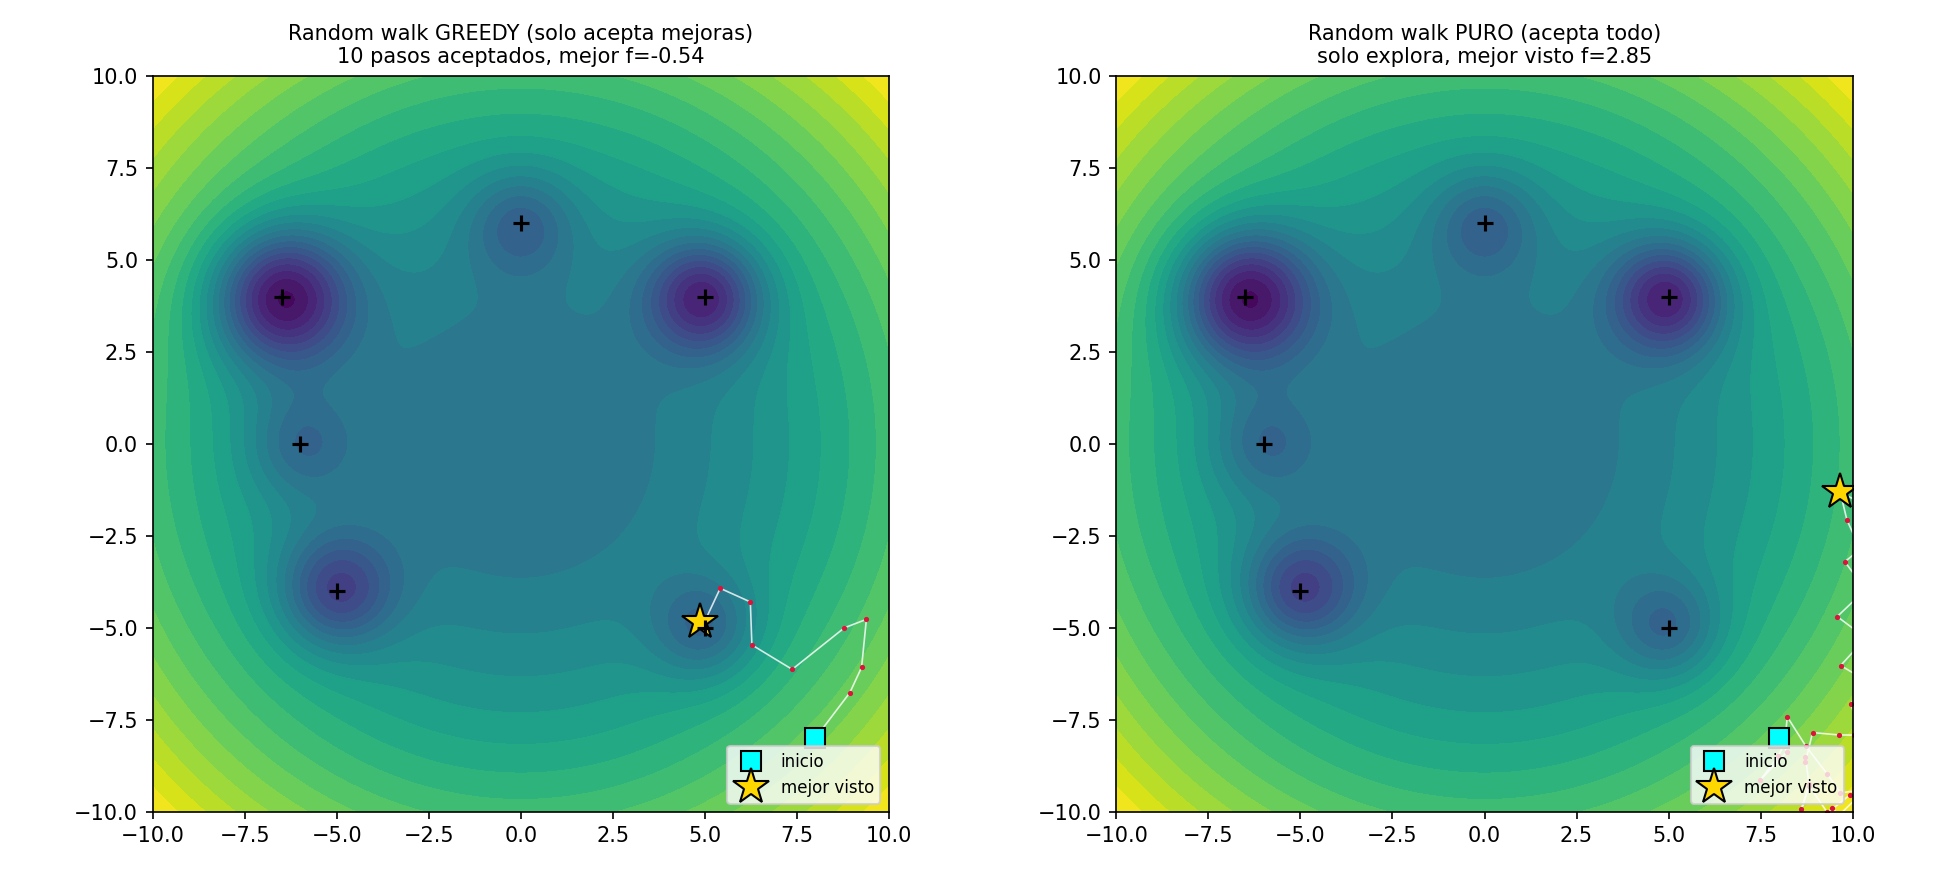
\includegraphics[width=0.92\textwidth,height=5.3cm,keepaspectratio]{fig05_random_walk.png}
  \end{center}
  \footnotesize Greedy (izq.): solo 10 de 500 pasos se aceptaron —
  encontró el pozo más cercano al punto de arranque y ya no pudo salir
  ($f=-0.54$, lejos del global $-3.29$). Puro (der.): se difunde sin
  rumbo, ni siquiera visita un pozo.
\end{frame}

\begin{frame}{Random walk: una lección incómoda}
  \begin{alertblock}{¿Y qué hizo Powell (el método "profesional" de scipy)?}
    Arrancando del mismo punto, \texttt{scipy.optimize.minimize(...,
    method="Powell")} converge a $(0,0)$ con $f\approx0$ — ¡el punto de
    "trampa" débil entre pozos, ni siquiera un mínimo real de los 6
    pozos! No encontró el mínimo global ($f=-3.29$).
  \end{alertblock}
  \begin{itemize}
    \item Ni el random walk greedy, ni Powell (un método local
      derivative-free serio), escapan solos de este paisaje con muchos
      mínimos locales.
    \item \textbf{Ningún optimizador puramente local} —con gradiente o
      sin él— tiene forma de "saber" que hay algo mejor del otro lado de
      una colina, si nunca la cruza.
    \item Por eso existen las \textbf{metaheurísticas} de la Clase 3:
      combinan un optimizador local con reinicios/aleatoriedad
      inteligente para tener más confianza de escapar de mínimos locales
      malos.
  \end{itemize}
\end{frame}

% ==================================================================
\section{Nelder--Mead (amoeba) en 2D}
% ==================================================================

\begin{frame}{Nelder--Mead: la idea}
  \begin{block}{Idea}
    Mantiene un \textbf{simplex} (en 2D: un triángulo, 3 puntos) y lo va
    deformando para "arrastrarlo" hacia el mínimo — como una ameba que
    cambia de forma para moverse. Es derivative-free y suele ser mucho
    más eficiente que grid search o random walk.
  \end{block}
  \begin{block}{Operaciones (ordenando los vértices: mejor $B$, medio,
    peor $P$; $C$=centroide sin $P$)}
    \begin{itemize}
      \item \textbf{Reflexión}: $R=C+(C-P)$. Si $f(R)$ mejora al mejor,
        probar \textbf{expansión} $E=C+2(R-C)$ (ir aún más lejos).
      \item Si $R$ mejora al segundo peor (pero no al mejor): aceptar $R$.
      \item Si no mejora nada: \textbf{contracción} hacia adentro
        $C_t=C+0.5(P-C)$.
      \item Si ni eso mejora: \textbf{encoger} todo el simplex hacia $B$.
    \end{itemize}
  \end{block}
\end{frame}

\begin{frame}[fragile]{Nelder--Mead: ejemplo paso a paso}
  $f(x,y)=x^2+2y^2$ (la de la Clase 1), arrancando de $(4,3)$:
  \tiny
\begin{lstlisting}
it= 1  mejor=[4. 3.] f=34.00000   peor=[4.  4.5] f=56.50000   REFLEXION
it= 2  mejor=[4. 3.] f=34.00000   peor=[5.5 3. ] f=48.25000   EXPANSION
it= 3  mejor=[3.25 0.75] f=11.68750   peor=[5.5 1.5] f=34.75000   REFLEXION
it= 5  mejor=[1. 0.] f=1.00000   peor=[1.75 2.25] f=13.18750   REFLEXION
it= 8  mejor=[1. 0.] f=1.00000   peor=[ 0.25 -2.25] f=10.18750   CONTRACCION
      ...
it=45  ->  x* = [-1.7e-05, -2.6e-05]   f(x*) = 1.61e-09
\end{lstlisting}
  \normalsize
  El simplex se refleja, expande cuando va por buen camino, y se
  contrae/encoge cuando se pasa — sin usar ninguna derivada.
\end{frame}

\begin{frame}{Nelder--Mead: evolución del simplex}
  \begin{center}
    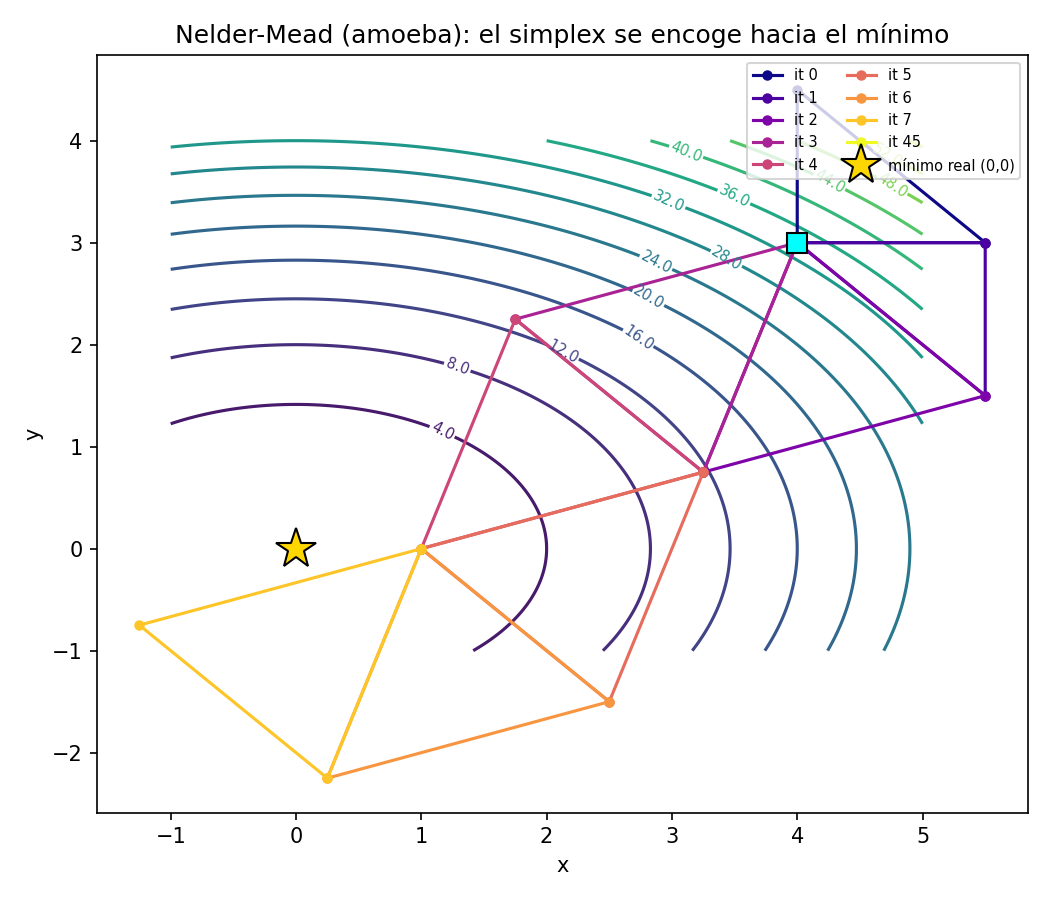
\includegraphics[height=6.2cm,keepaspectratio]{fig06_nelder_mead.png}
  \end{center}
\end{frame}

\begin{frame}[fragile]{Nelder--Mead: código}
  \begin{columns}
    \column{0.55\textwidth}
    \textbf{Manual (núcleo, un paso):}
\begin{lstlisting}
simplex.sort(key=f)
B, *resto, P = simplex
C = np.mean(simplex[:-1], axis=0)
R = C + (C - P)                    # reflexion
if f(R) < f(B):
    E = C + 2*(R - C)              # expansion
    simplex[-1] = E if f(E)<f(R) else R
elif f(R) < f(resto[-1]):
    simplex[-1] = R
else:
    Ct = C + 0.5*(P - C)           # contraccion
    if f(Ct) < f(P): simplex[-1] = Ct
    else: simplex = [B+0.5*(v-B) for v in simplex]
\end{lstlisting}
    \column{0.45\textwidth}
    \textbf{Con scipy:}
\begin{lstlisting}
from scipy.optimize import minimize

res = minimize(
    f, x0,
    method="Nelder-Mead")
\end{lstlisting}
    \small Manual: 45 iteraciones,
    $f^*=1.6\times10^{-9}$. \\
    Scipy: 75 iteraciones,
    $f^*=2.8\times10^{-17}$ (usa
    tolerancias internas más
    estrictas y ajustes finos que
    la versión didáctica de aquí).
  \end{columns}
  \vspace{0.2cm}
  Script completo: \texttt{scripts/06\_nelder\_mead\_2d.py}
\end{frame}

% ==================================================================
\section{Síntesis}
% ==================================================================

\begin{frame}{Comparación de los 5 métodos}
  \tiny
  \begin{center}
  \begin{tabular}{lccccc}
    \toprule
    & \textbf{Bisección} & \textbf{Áurea} & \textbf{Grid search} &
      \textbf{Random walk} & \textbf{Nelder--Mead} \\
    \midrule
    Variables & 1 & 1 & 1--3 (práctico) & cualquiera & cualquiera \\
    Usa $f'$ & sí & no & no & no & no \\
    Determinista & sí & sí & sí & no (parcial) & sí \\
    Garantiza mínimo & local, & local, & de la malla & no & local \\
    (con supuestos) & si unimodal & si unimodal & (converge si $N\to\infty$) & & \\
    Costo & $O(\log(1/\epsilon))$ & $O(\log(1/\epsilon))$ & $O(N^d)$ &
      $O(\text{iter})$, ineficiente & $O(\text{iter})$, eficiente \\
    Cuándo usarlo & $f'$ barata, & $f$ costosa/no & pocas variables, & casi
      nunca solo & muchas variables, \\
    & 1 variable & diferenciable & sin garantías & (sirve de base & sin
      derivadas, \\
    & & & sobre $f$ & para Clase 3) & robusto \\
    \bottomrule
  \end{tabular}
  \end{center}
\end{frame}

\begin{frame}{Lo que tienen en común}
  \begin{block}{}
    Todos comparten una limitación importante: son (o dependen
    fuertemente de ser) \textbf{métodos locales} o de \textbf{costo
    exponencial}. Ninguno de los cinco, tal como los vimos hoy, tiene una
    estrategia inteligente para escapar de un mínimo local malo en un
    paisaje con muchos pozos, sin pagar el precio exponencial del grid
    search.
  \end{block}
  \begin{exampleblock}{La pregunta que abre la Clase 3}
    ¿Cómo combinamos la eficiencia de un optimizador local (como
    Nelder--Mead) con la capacidad de \textbf{escapar} de mínimos locales
    (como random walk, pero de forma más inteligente)?
  \end{exampleblock}
\end{frame}

% ==================================================================
\section{Vista previa: Clase 3}
% ==================================================================

\begin{frame}{Clase 3: metaheurísticas}
  \begin{itemize}
    \item \textbf{Basin hopping}: alterna reoptimización local (como
      Nelder--Mead) con saltos aleatorios (como random walk) y un
      criterio de aceptación tipo Metrópolis.
    \item \textbf{Simulated annealing}: el mismo criterio de Metrópolis,
      pero con una "temperatura" que baja con el tiempo — mucha
      exploración al inicio, mucha explotación al final.
    \item \textbf{Algoritmos genéticos}: una \textbf{población} de
      soluciones que evoluciona por selección, cruce y mutación.
    \item \textbf{Particle swarm optimization}: un \textbf{enjambre} de
      partículas que se mueven influenciadas por su mejor posición y la
      del grupo.
  \end{itemize}
  \vspace{0.3cm}
  \begin{alertblock}{}
    Todos, otra vez, con código manual \textbf{y} su equivalente en
    scipy (donde exista) para comparar.
  \end{alertblock}
\end{frame}

% ==================================================================
\section{Ejercicios propuestos}
% ==================================================================

\begin{frame}{Ejercicios para la próxima clase}
  \small
  \begin{enumerate}
    \item Use bisección para minimizar $f(x)=x^4-3x^2+x$ en un intervalo
      donde $f'$ cambie de signo. Verifique con \texttt{scipy.optimize.brentq}.
    \item Compare, para tres tolerancias distintas ($10^{-3},10^{-6},
      10^{-9}$), cuántas iteraciones necesitan bisección y búsqueda
      áurea. ¿La diferencia crece o se mantiene constante?
    \item Implemente grid search en 4 variables para
      $f(x_1,x_2,x_3,x_4)=\sum x_i^2$ con $N=20$ puntos por eje. Mida el
      tiempo de ejecución y compárelo con el caso $N=20,d=2$.
    \item Modifique \texttt{scripts/05\_random\_walk\_2d.py} agregando un
      \emph{reinicio}: si tras 50 pasos no hay mejora, saltar a un punto
      aleatorio nuevo. Compare el resultado contra la versión sin
      reinicios.
    \item Modifique \texttt{scripts/06\_nelder\_mead\_2d.py} para
      $f(x,y)=(x-2)^2+(y+1)^2 + 5\sin(x)\cos(y)$ (no convexa) y observe si
      el simplex encuentra el mínimo global o queda atrapado.
    \item Para el paisaje de 6 pozos (\texttt{scripts/\_landscape.py}),
      corra grid search 2D con $N=10,25,50,100$ y grafique el error
      respecto al mínimo verdadero vs.\ el número de evaluaciones.
    \item \textbf{Reflexión:} explique con sus palabras por qué Nelder--Mead
      normalmente necesita muchas menos evaluaciones que grid search para
      la misma precisión, y en qué casos esa ventaja desaparece.
  \end{enumerate}
\end{frame}

% ==================================================================
\section{Referencias}
% ==================================================================

\begin{frame}{Referencias}
  \footnotesize
  \begin{itemize}
    \item J. Nocedal, S. Wright. \emph{Numerical Optimization}, 2.\textsuperscript{a}
      ed. Springer, 2006.
    \item M. Kochenderfer, T. Wheeler. \emph{Algorithms for Optimization}.
      MIT Press, 2019. (Cubre bisección, áurea, Nelder--Mead y búsquedas
      estocásticas con código.)
    \item W. Press, S. Teukolsky, W. Vetterling, B. Flannery.
      \emph{Numerical Recipes}, 3.\textsuperscript{a} ed. Cambridge
      University Press, 2007. (Capítulo 10: minimización 1D y
      multidimensional.)
    \item J. Nelder, R. Mead. "A Simplex Method for Function
      Minimization." \emph{Computer Journal}, 7(4), 1965.
    \item D. Boyd, J. Vandenberghe. \emph{Convex Optimization}.
      Cambridge University Press, 2004.
    \item Documentación de \texttt{SciPy}
      (\texttt{scipy.optimize}): \url{https://scipy.org}.
  \end{itemize}
\end{frame}

\begin{frame}[standout]
  ¿Preguntas?
\end{frame}

\end{document}
